\begin{chapter}{Protótipo}
O acionador baseado em sopro foi desenvolvido com a intenção de ser
\textit{open-source} e de baixo custo, para que mais pessoas possam ter acesso
a essa ferramenta que pode ser utilizada como método alternativo para o clique
do \textit{mouse}. O circuito do protótipo desenvolvido neste trabalho é mostrado 
na Figura~\ref{fig:circuito}

\begin{figure}[!h]
	\centering
	\begin{minipage}[c]{\textwidth}
	\centering
	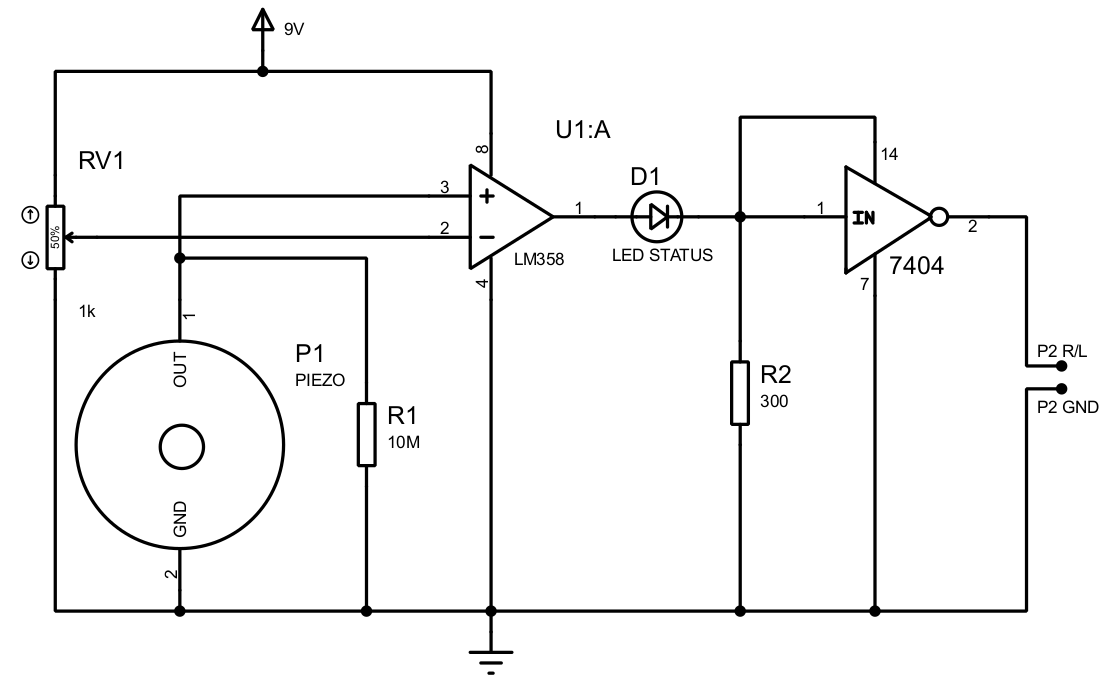
\includegraphics[width=1\linewidth]{fig/acionador}
	\caption{Esquemático do acionador baseado em sopro.}
	\label{fig:circuito}
	\end{minipage}
\end{figure} 

O princípio de funcionamento do acionador exeterno proposto é relativamente
simples. A percepção do sopro é realizada graças ao piezo encapsulado em um
disco redondo que fica acoplado na parte superior do dispositivo. Quando o
usuário realiza o sopro diretamente no piezo, há um estresse mecânico que produz
uma diferança de potencial nas extremidades do material piezoelétrico. Atráves
da percepção dessa tensão produzida no piezo é possível gerar um evento de
clique de \textit{mouse} no computador. O resistor colocado em paralelo com o
piezo é responsável por determinar a sensibilidade com que o transdutor gera
tensão após ser submetido a algum tipo de estresse mecânico. Portanto quanto
maior o valor de resistência do resistor, maio será a sensibilidade do piezo.
No protótipo desenvolvido utilizou-se um resistor de 10~M\si{\ohm} o que
proporcionou uma boa sensibilidade no piezo. Foram testados resistores com
valores de resistência maior que 10~M\si{\ohm}, como 15~M\si{\ohm}, 20~M\si{\ohm} e
30~M\si{\ohm}, contudo a sensibilidade com resistência maiores que 15~M\si{\ohm}
deixava o transdutor muito suscetível a detectar estresses mecânicos com
intensidades não desejadas. Já resistências menores que 15~M\si{\ohm} não
alterava significamente a sensibilidade do piezo, quando comparado com o
resistor de 10~M\si{\ohm}. 

O sinal da tensão gerado nas extremidas do material piezoelétrico é analógico.
Contudo, como o clique do \textit{mouse} possui uma natureza binária, pois há
apenas dois estados possíveis --- clique ativado e clique não ativado ---, não
seria possível utilizar diretamente essa tensão produzida como forma de ativação
do clique devido a grande quantidade de ruído que esse sinal possui, como
mostrado na Figura~\ref{fig:ruido}. Por isso houve a necessidade de digitalizar
a saída do acionador.

A solução encontrada para relizar a tarefa de ``converter'' o sinal analógico
do acionador para um sinal digital, foi a utilização de um amplificador
operacional LM358. Esse componente eletrônico possui a função de comparar duas
tensões que determinam a saída do acionador. Há uma tensão de referência
, que pode ser varivável graças a um potenciômetro de 10~k\si{\ohm}, e a tensão
produzida pelo transdutor piezo. O amplificador operacional atua, neste caso,
como um comparador de tensões. Quando a tensão de referência é superior a tensão
do piezo, a saida do aplificador é de nivel lógigo baixo. Contudo, quando a
tensão de referência é inferior a tensão do piezo, a saída do amplificador é de
nivel lógico alto. Não há possibilidade de a saída do amplificador ser diferente
desses dois casos. Dessa forma, a leitura do sinal de tensão produzido pelo sopro
, com o auxílio do piezo, é binária, o que ajuda a implementar a emulação dos
eventos de clique. É importante ressaltar que como o valor de referência 
pode ser ajustável graças ao potenciômetro, esse componente também atua como um
ferramenta de ajuste de sensibilidade. Sendo assim, a intensidade do sopro
necessária para que a saída do amplificador seja de nível lógico alto,
configurando assim um clique, pode ser determinada pela tensão de referência
ajustada pelo potenciômetro.

\end{chapter}
